\documentclass{article}
\usepackage{eecstex}
\usepackage{pgfplots}

\title{EE 120 HW 02}
\author{Bryan Ngo}
\date{2021-01-30}

\begin{document}

\maketitle

\section{Continuous Time System Properties}

\subsection{}

\begin{equation}
    y(t) = x(t - 2) + x(2 - t)
\end{equation}
Let \(y_1(t) = x_1(t - 2) + x_1(2 - t)\) and \(y_2(t) = x_2(t - 2) + x_2(2 - t)\).
\textbf{Proving linearity}, let \(x(t) = \alpha x_1(t) + \beta x_2(t)\),
\begin{align}
    y(t) = x(t - 2) + x(2 - t) &= \alpha x_1(t - 2) + \beta x_2(t - 2) + \alpha x_1(2 - t) + \beta x_2(2 - t) \\
    &= \alpha (x_1(t - 2) + x_2(2 - t)) + \beta (x_2(t - 2) + x_2(2 - t)) \\
    &= \alpha y_1(t) + \beta y_2(t)
\end{align}
\textbf{Disproving time invariance},
\begin{equation}
    x((t - t_0) - 2) + x(2 - (t - t_0)) = x(t - t_0 - 2) + x(2 - t + t_0) \neq y(t - t_0)
\end{equation}
The system is \textbf{not memoryless or causal}, since, for example, \(y(0)\) depends on \(x(-2)\) and \(x(2)\).
\textbf{Proving stability}, let \(\max_x\{|x(t)|\} = B_x\), then \(y(t) \leqslant B_x + B_x = 2B_x\).

\subsection{}

\begin{equation}
    y(t) = x(t / 3)
\end{equation}
Let \(y_1(t) = x_1(t / 3)\) and \(y_2(t) = x_2(t / 3)\).
\textbf{Proving linearity}, let \(x(t) = \alpha x_1(t) + \beta x_2(t)\),
\begin{equation}
    y(t) = \alpha x_1(t / 3) + \beta x_2(t / 3) = \alpha y_1(t) + \beta y_2(t)
\end{equation}
\textbf{Disproving time invariance},
\begin{equation}
    x((t - t_0) / 3) \neq y(t - t_0) = x(t / 3 - t_0)
\end{equation}
The system is \textbf{not memoryless}, since, for example, \(y(1)\) depends on \(x(1 / 3)\).
The system is \textbf{not causal}, since, for example, \(y(-1)\) depends on \(x(-1 / 3)\).
\textbf{Proving stability}, let \(\max_x\{|x(t)|\} = B_x\), then \(y(t) \leqslant B_x\).

\subsection{}

\begin{equation}
    y(t) = x(t) \cos(5t)
\end{equation}
Let \(y_1(t) = x_1(t) \cos(5t)\) and \(y_2(t) = x_2(t) \cos(5t)\).
\textbf{Proving linearity}, let \(x(t) = \alpha x_1(t) + \beta x_2(t)\),
\begin{equation}
    y(t) = \cos(5t) (\alpha x_1(t) + \beta x_2(t)) = \alpha x_1(t) \cos(5t) + \beta x_2(t) \cos(5t) = \alpha y_1(t) + \beta y_2(t)
\end{equation}
\textbf{Disproving time invariance},
\begin{equation}
    x(t - t_0) \cos(5 (t - t_0)) \neq y(t - t_0) = x(t - t_0) \cos(5t - t_0)
\end{equation}
The system is \textbf{memoryless}, since there is not scaling or delay of the input signal's time.
The system is \textbf{causal}, since all memoryless systems are also causal.
\textbf{Proving stability}, let \(\max_x\{|x(t)|\} = B_x\), then \(|y(t)| \leqslant B_x\), since the cosine function's range is \([-1, 1]\).

\section{Discrete Time System Properties}

\subsection{}

\begin{equation}
    y[n] = \sum_{k \in [1, n]} x[k]
\end{equation}
Let \(y_1[n] = \sum_{k \in [1, n]} x_1[k]\) and \(y_2[n] = \sum_{k \in [1, n]} x_2[k]\).
\textbf{Proving linearity}, let \(x[n] = \alpha x_1[n] + \beta x_2[n]\),
\begin{align}
    y[n] = \sum_{k \in [1, n]} x[k] &= \sum_{k \in [1, n]} \alpha x_1[k] + \beta x_2[k] \\
    &= \alpha \sum_{k \in [1, n]} x_1[k] + \beta \sum_{k \in [1, n]} x_2[k] \\
    &= \alpha y_1[n] + \beta y_2[n]
\end{align}
\textbf{Proving time invariance},
\begin{equation}
    \sum_{k \in [1, n - n_0]} x[k] = y[n - n_0]
\end{equation}
The system is \textbf{not memoryless}, since the sum is inherently dependent on past values of \(x[k]\).
The impulse response is
\begin{equation}
    h[n] = \sum_{k \in [1, n]} \delta[k] = 0
\end{equation}
assuming \(n \geqslant 1\).

\subsection{}

\begin{equation}
    y[n] = \sum_{k \in [0, 4]} (-1)^k x[n - k]
\end{equation}
Let \(y_1[n] = \sum_{k \in [0, 4]} (-1)^k x_1[n - k]\) and \(y_2[n] = \sum_{k \in [0, 4]} (-1)^k x_2[n - k]\).
\textbf{Proving linearity}, let \(x[n] = \alpha x_1[n] + \beta x_2[n]\),
\begin{align}
    y[n] = \sum_{k \in [0, 4]} (-1)^k x[n - k] &= \sum_{k \in [0, 4]} (-1)^k \left(\alpha x_1[n - k] + \beta x_2[n - k]\right) \\
    &= \alpha \sum_{k \in [0, 4]} (-1)^k x_1[n - k] + \beta \sum_{k \in [0, 4]} (-1)^k x_2[k] \\
    &= \alpha y_1[n] + \beta y_2[n]
\end{align}
\textbf{Proving time invariance},
\begin{equation}
    \sum_{k \in [0, 4]} (-1)^k x[(n - n_0) - k] = y[n - n_0]
\end{equation}
The system is \textbf{not memoryless}, since, for example, \(y[0]\) depends on \(x[-1]\).
The impulse response is
\begin{equation}
    h[n] = \sum_{k \in [0, 4]} (-1)^k \delta [n - k] = \delta[n] - \delta[n - 1] + \delta[n - 2] - \delta[n - 3] + \delta[n - 4] 
    \begin{cases}
        1 & n = 0, 2, 4 \\
        -1 & n = 1, 3 \\
        0 & \text{elsewhere}
    \end{cases}
\end{equation}

\subsection{}

\begin{equation}
    y[n] = \cos[x[n] + \tfrac{\pi}{3}]
\end{equation}
Let \(y_1[n] = \cos[x_1[n] + \tfrac{\pi}{3}]\) and \(y_2[n] = \cos[x_2[n] + \tfrac{\pi}{3}]\).
\textbf{Disproving linearity}, perform the \(a = 0\) test,
\begin{equation}
    y[n] = \cos[0 \cdot x[n] + \tfrac{\pi}{3}] = \cos[\tfrac{\pi}{3}] \neq 0
\end{equation}
\textbf{Proving time invariance},
\begin{equation}
    \cos[x[n - n_0] + \tfrac{\pi}{3}] = y[n - n_0]
\end{equation}
The system is \textbf{memoryless}, since \(y[n]\) only depends on \(x[n]\).

\subsection{}

\begin{equation}
    y[n] = x[n] + \frac{1}{2} (x[n - 1])^2
\end{equation}
Let \(y_1[n] = x_1[n] + \frac{1}{2} (x_1[n - 1])^2\) and \(y_2[n] = x_2[n] + \frac{1}{2} (x_2[n - 1])^2\).
\textbf{Disproving linearity}, let \(x[n] = \alpha x_1[n] + \beta x_2[n]\),
\begin{align}
    y[n] &= \alpha x_1[n] + \beta x_2[n] + \frac{1}{2} (\alpha x_1[n - 1] + \beta x_2[n - 1])^2 \\
    &\neq \alpha \left(x_1[n] + \frac{1}{2} (x_1[n - 1])^2\right) + \beta \left(x_2[n] + \frac{1}{2} (x_2[n - 1])^2\right)
\end{align}
\textbf{Proving time invariance},
\begin{equation}
    x[n - n_0] + \frac{1}{2} (x[(n - n_0) - 1])^2 = y[n - n_0]
\end{equation}
The system is \textbf{not memoryless}, since \(y[n]\) depends on \(x[n - 1]\).

\section{Discrete Time Infinite Impulse Response Filter}

\begin{equation}
    y[n] = \alpha y[n - N] + x[n]
\end{equation}

\subsection{}

\begin{center}
    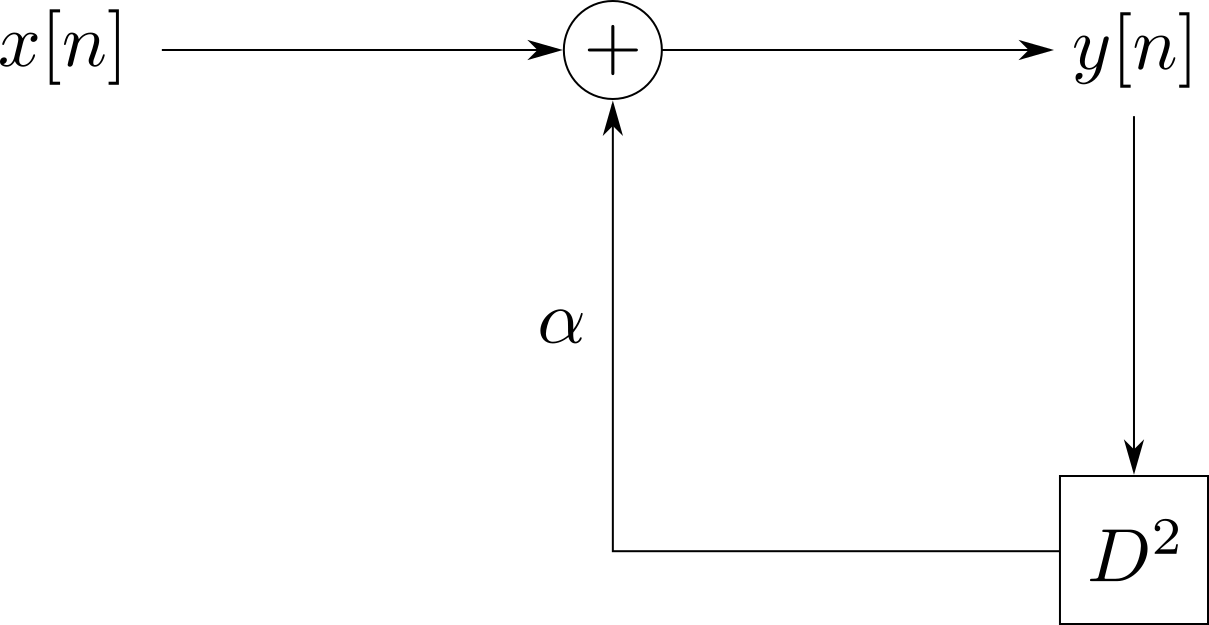
\includegraphics[width=0.7\textwidth]{q3-1.png}
\end{center}

\subsection{}

In the homogeneous case, assume the solution is in the form \(y_h[n] = A \lambda^n\).
Then,
\begin{align}
    A\lambda^n - \alpha A \lambda^{n - N} &= 0 \\
    1 - \alpha \lambda^{-N} &= 0 \\
    \Rightarrow \lambda = \alpha^{\frac{1}{N}} &\implies y_h[n] = A \alpha^{\frac{n}{N}}
\end{align}
Finding the particular solution, consider the following time step and outputs:
\begin{equation}
    \begin{array}[]{||c|c||}
        \hline
        n & f_p[n] \\
        \hline
        0 & f[0] - \alpha \cancelto{0}{f[-N]} = 1 \\
        N & f[N] = \alpha f[0] = \alpha \\
        2N & f[2N] = \alpha f[N] = \alpha^2 \\
        \vdots & \vdots \\
        \hline
    \end{array}
\end{equation}
Meaning that \(f_p[n] = \alpha^{\frac{n}{N}}u[n]\).
Our general solution is \(f[n] = \alpha^{\frac{n}{N}} (A + u[n])\).
Given the initial condition \(f[-1] = 0\),
\begin{equation}
    0 = A \alpha^{-\frac{1}{N}} \implies A = 0
\end{equation}
giving us a final equation of \(f[n] = \alpha^{\frac{n}{N}} u[n]\).

\subsection{}

\begin{center}
    \begin{tikzpicture}
        \begin{axis}[
            xlabel=\(n\), ylabel={\(f[n]\)},
            title={DT IIR Filter (\(\alpha = \frac{1}{2}, N = 2\))},
            axis lines=middle,
            ymin=0, ymax=1,
            width=0.4\textwidth
        ]
        \addplot[ycomb, mark=*, color=blue] table[
            col sep=comma,
            x=n, y=3a
        ]{q3-3.csv};
        \end{axis}
    \end{tikzpicture}
    \begin{tikzpicture}
        \begin{axis}[
            xlabel=\(n\), ylabel={\(f[n]\)},
            title={DT IIR Filter (\(\alpha = \frac{1}{\sqrt{2}}, N = 2\))},
            axis lines=middle,
            ymin=0, ymax=1,
            width=0.4\textwidth
        ]
        \addplot[ycomb, mark=*, color=blue] table[
            col sep=comma,
            x=n, y=3b
        ]{q3-3.csv};
        \end{axis}
    \end{tikzpicture}
    \begin{tikzpicture}
        \begin{axis}[
            xlabel=\(n\), ylabel={\(f[n]\)},
            title={DT IIR Filter (\(\alpha = \frac{1}{2}, N = 4\))},
            axis lines=middle,
            ymin=0, ymax=1,
            width=0.4\textwidth
        ]
        \addplot[ycomb, mark=*, color=blue] table[
            col sep=comma,
            x=n, y=3c
        ]{q3-3.csv};
        \end{axis}
    \end{tikzpicture}
\end{center}
The value \(\alpha\) affects how steep the decay of the system is, and \(N\) has the same effect.

\subsection{}

The equation is
\begin{equation}
    y[n] = y[n - 1] + u[n]
\end{equation}
The homogeneous response, given our parameters, is simply \(y_h[n] = A\).
The particular response is
\begin{equation}
    \begin{array}[]{||c|c||}
        \hline
        n & y_p[n] \\
        \hline
        0 & f[0] = \cancelto{0}{f[-N]} + 1 = 1 \\
        1 & f[1] = f[0] + 1 = 2 \\
        2 & f[2] = f[1] + 1 = 3 \\
        \vdots & \vdots \\
        \hline
    \end{array}
\end{equation}
giving us a particular solution of \(y_p[n] = (n + 1) u[n]\).
The general formula is \(y[n] = A + (n + 1) u[n]\).
Given the initial condition \(y[-1] = 0\), we get that \(A = 0\), so \(y[n] = (n + 1) u[n]\).

\section{Continuous Time LCCDE Practice}

\begin{equation}
    \diff{t} y(t) + \frac{1}{3} y(t) = x(t)
\end{equation}

\subsection{}

\begin{equation}
    \diff{t} y_h(t) + \frac{1}{3} y_h(t) = 0 \implies y_h(t) = A e^{-\frac{1}{3} t}
\end{equation}

\subsection{}

\begin{equation}
    \diff{t} y_p(t) + \frac{1}{3} y_p(t) = e^{-t} u(t)
\end{equation}
When \(t < 0\), \(y_p(t) = 0\) due to the nature of the unit step function.
When \(t \geqslant 0\),
\begin{equation}
    \diff{t} y_p(t) + \frac{1}{3} y_p(t) = e^{-t}
\end{equation}
By inspection, we find that \(y_p(t) = -\frac{3}{2} e^{-t} u(t)\).

\subsection{}

\begin{equation}
    y(t) = A e^{-\frac{1}{3}t} - \frac{3}{2} e^{-t} u(t)
\end{equation}

\subsection{}

Since the homogeneous solution is input-dependent, \(\hat{y}_h(t) = A e^{-\frac{1}{3} (t - T)}\).
We are allowed to make such a substitution because shifting a variable does not change its derivative according to the chain rule.
Finding the particular solution for \(t \geqslant T\),
\begin{equation}
    \diff{t} \hat{y}_p(t) + \frac{1}{3} \hat{y}_p(t) = e^{-(t - T)}
\end{equation}
Then, we find that \(\hat{y}_p(t) = -\frac{3}{2} e^{-(t - T)} u(t - T)\).
Our final output is
\begin{equation}
    \hat{y}(t) = A e^{-\frac{1}{3}(t - T)} - \frac{3}{2} e^{-(t - T)} u(t - T) = y(t - T)
\end{equation}

\section{Block Diagram Practice}

\subsection{}

\begin{equation}
    y[n] = r[n] + r[n - 1] = x[n] - 2r[n - 1] + r[n - 1] = x[n] - r[n - 1]
\end{equation}

\subsection{}

Yes, the system is an LTI system.

\subsection{}

No, the system is dependent on \(r[n + 2]\).

\subsection{}

\subsection{}

\subsection{}

\end{document}
